\subsection{Bot Comparison Tool} 
\begin{figure}[htbp]
    \centering
    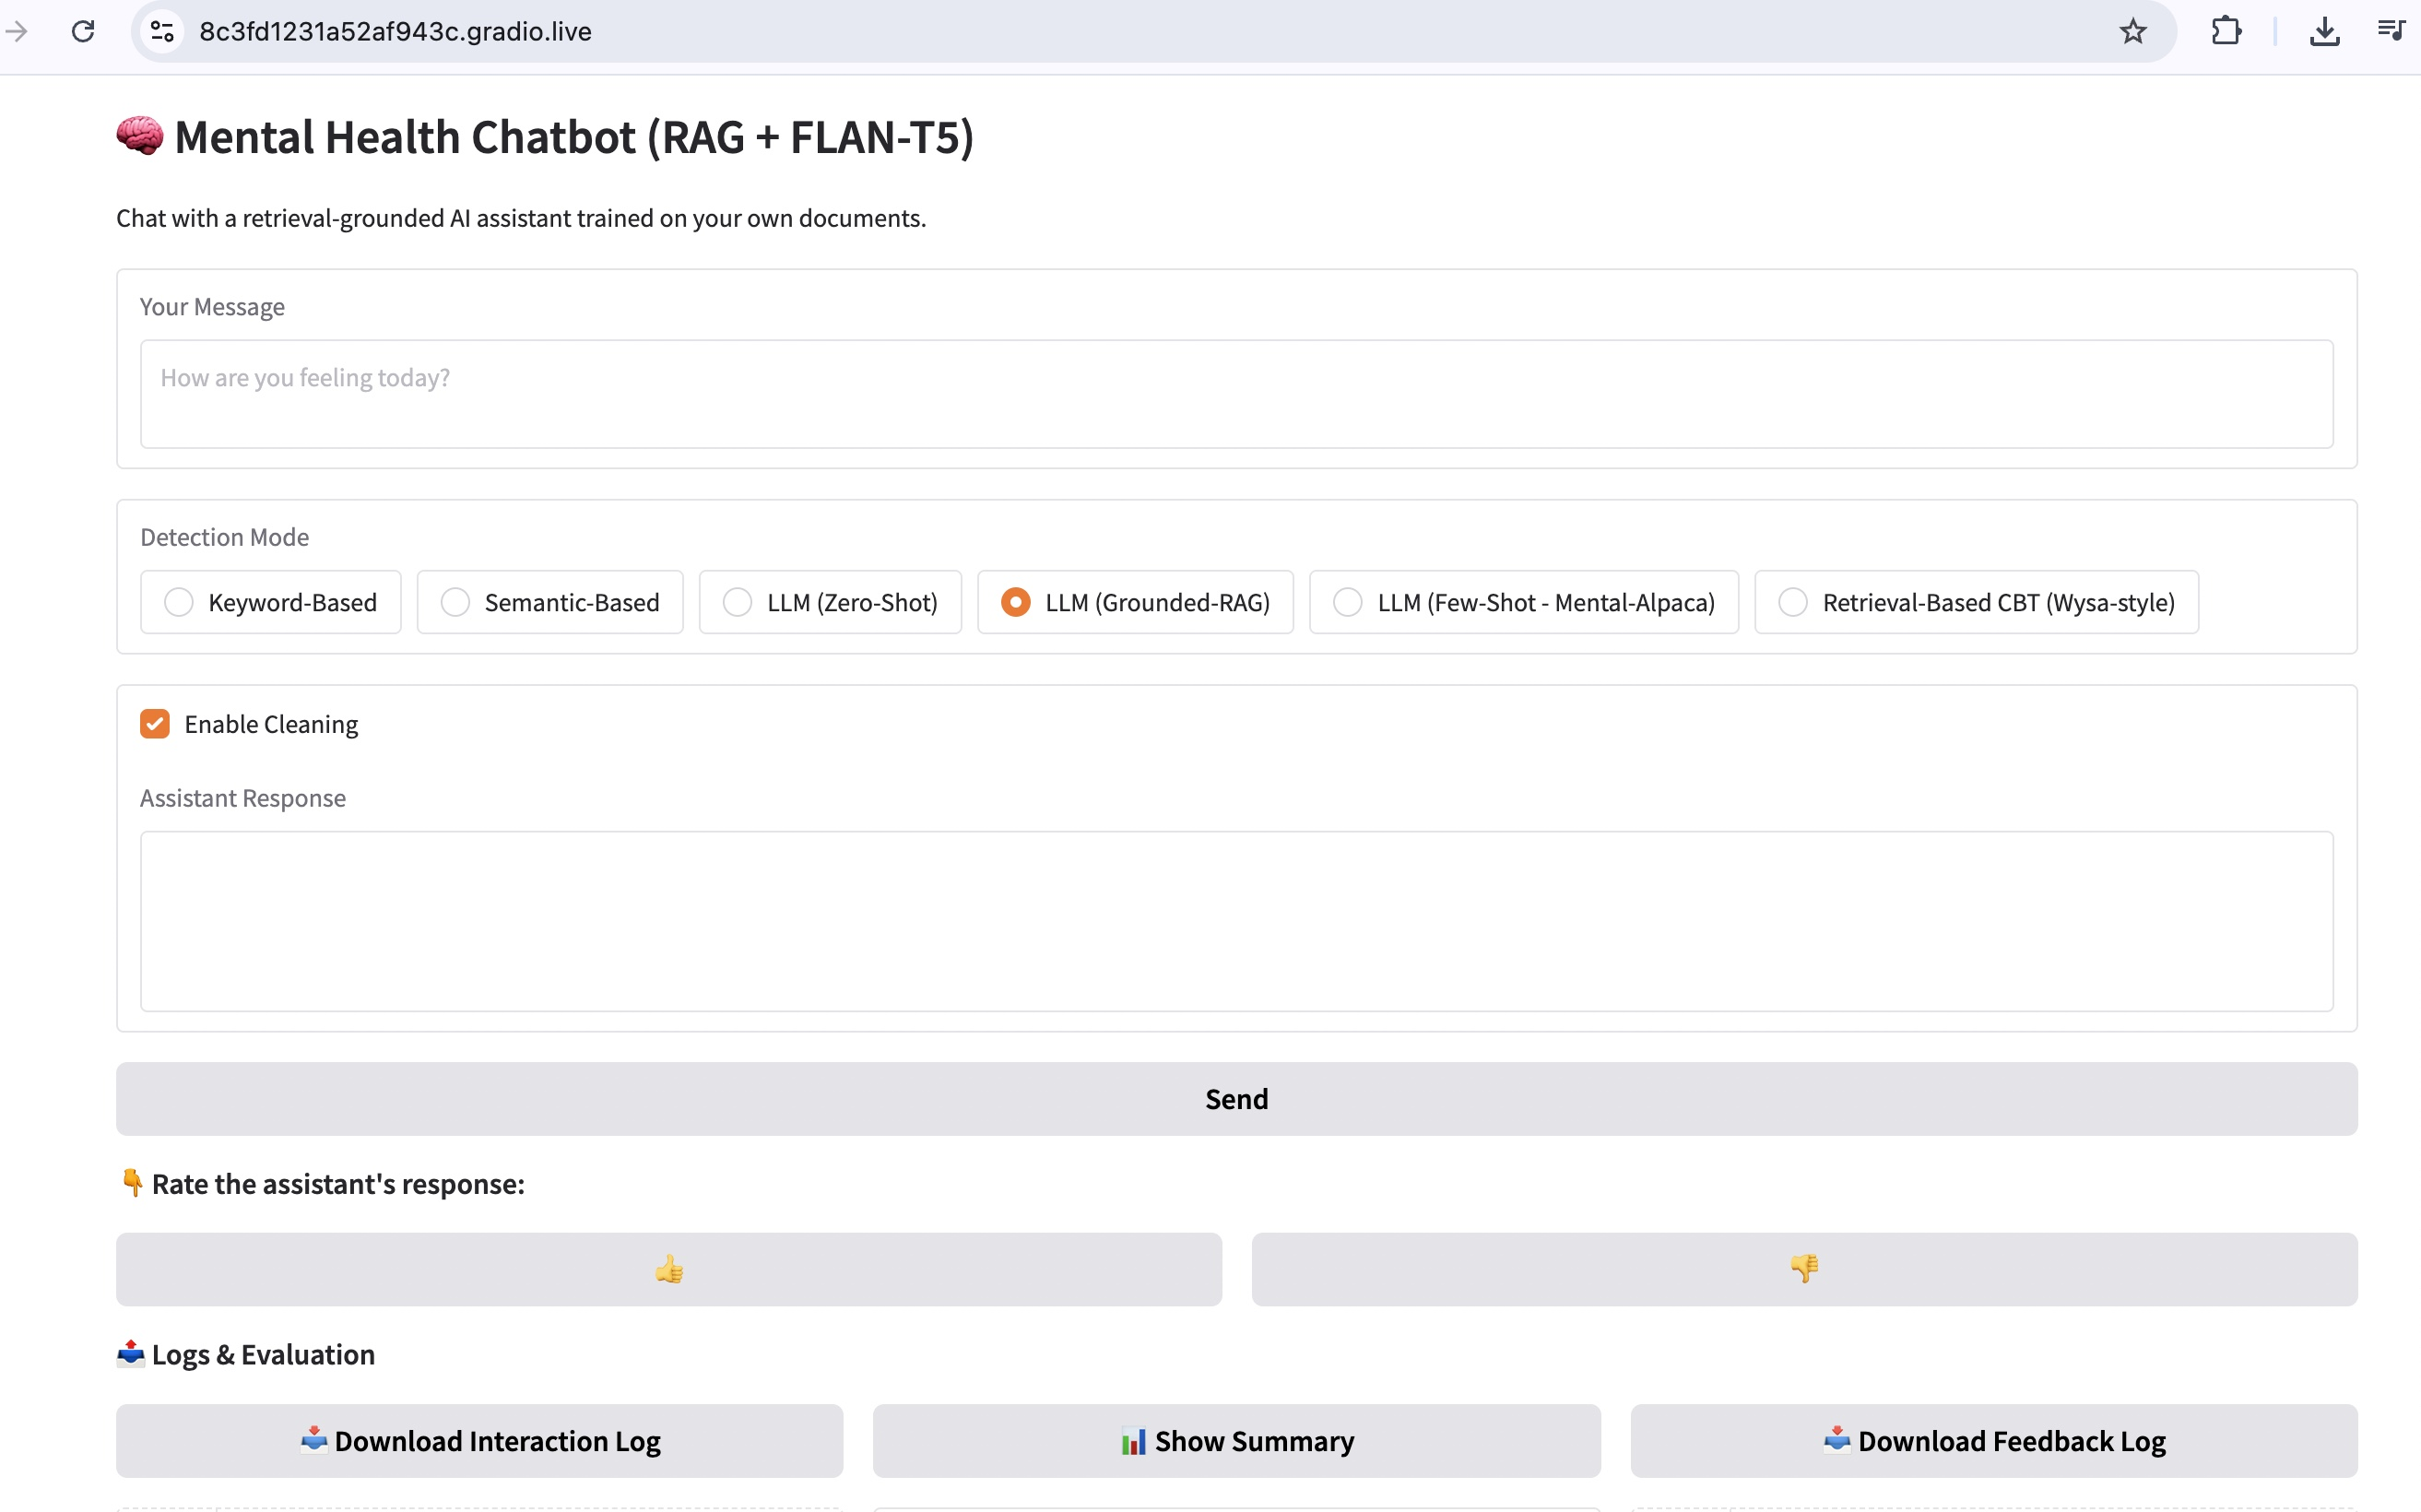
\includegraphics[width=0.8\textwidth]{bot_comparison_tool.jpeg}
    \caption{Comparison tool of Different Types of Mental Health Chatbots}
    \label{fig:bot_comparison}
\end{figure}
We built this comparison to help understand the different types of mental health chatbots described in the literature. By analyzing models like keyword-based bots, semantic-based bots, zero-shot models, grounded models and CBT-based bots, we evaluated their strengths and weaknesses in handling mental health queries. This comparison aligns with the findings from the literature, showcasing how different approaches, from simple keyword matching to complex retrieval-augmented generation and fine-tuned models, offer varying degrees of empathy, accuracy, and context-awareness but the responses offered were questionable in a lot of contexts. 





\subsection{Dataset Impact Comparison} 
This dataset presents a comparative analysis of three chatbot models built upon the GPT-2 base architecture (nsbarla/gpt2-base), each fine-tuned with different training data to explore their responsiveness to emotionally sensitive prompts. One model was trained on a Reddit dataset (nsbarla/gpt2-reddit), another on empathy-rich conversations from Hugging Face (nsbarla/gpt2-empathy) and the third remained as the unaltered baseline. All three models were exposed to the same set of ten distress-related prompts, and their outputs were recorded for comparison. The responses are unique across the models, offering insight into how different training influences affect tone, empathy, and coherence. The empathy-tuned model generally strives to offer supportive or compassionate replies, although some are shallow or lack contextual depth. The Reddit-style model frequently mirrors informal, narrative-driven responses, occasionally incorporating anecdotal elements reflective of real-world user conversations. Conversely, the vanilla model often produces short, vague, or incomplete outputs, indicating limited emotional understanding and generative capacity. Collectively, the dataset reveals distinct stylistic and qualitative differences, shedding light on how training data shapes a model’s ability to engage with sensitive or personal topics.
\begin{table}[H]
    \centering
    \tiny
    \resizebox{\textwidth}{!}{%
    \begin{tabular}{|p{3cm}|p{3cm}|p{3cm}|p{3cm}|}
        \toprule
        \hline
        Prompt & Base Response & Reddit Response & Empathy Response \\
        \hline
        \midrule
        \hline
        I'm feeling really down lately. I don't want to wake up. & I was really & So I'm just going to be taking a shower and eating food. & I am sorry. I hope you can find a new job soon. \\
        \hline
        No one listens to me when I say I'm not okay. & No, I don't care. & No one listens to me when I say I'm not okay. & I'm sorry, I would be so mad at you. \\
        \hline
        I feel like I'm a burden to everyone around me. & I don't want to be on the wrong side of the spectrum. I want to be a person who wants to be respected and respected and respected by all of the other people who don't really understand how I'm supposed to be. I want to be a person who believes in a person who believes in & I feel like I'm an annoying burden to everybody around me. & Oh no \\
        \hline
        I don't know if I can keep going. & I can & I am a social-exchange student and I have a really low self-esteem. & I have a small dog that's just a little bit older. I can't do much about it. \\
        \hline
        I want to feel better, but I can't see a way out. & I want to & I'm doing this because I don't want to be seen as a piece of shit. I just want to be happy. I want to be happy. I want to be happy.  & I was in a housework meeting and saw a big group of people trying to make a sandwich. \\
        \hline
        \bottomrule
    \end{tabular}%
    }
\end{table}


\subsection{Fine-tuned Chatbot with LoRa} 
The Mistral-7B-Instruct-v0.1 model, fine-tuned on a mental health dataset and optimized using LoRA and 4-bit quantization, is now available on Hugging Face under the model ID nsbarla/mental-health-mistral-lora. It was trained on Hugging Face's platform using GPUs, a process that took over 2-3 hours due to the model's size and the applied optimizations. This fine-tuned model is designed to offer more efficient and contextually relevant responses for conversations related to mental health, making it an ideal resource for applications aiming to support users in need of empathetic interactions and advice.
The Mistral Mental Health Bot was trained on a combined dataset consisting of Empathetic Dialogues and Counsel Chat datasets. The Empathetic Dialogues dataset includes conversations designed to encourage empathetic and supportive responses, while the Counsel Chat dataset contains counseling-style dialogues aimed at addressing mental health concerns.
\begin{figure}[h]
    \centering
    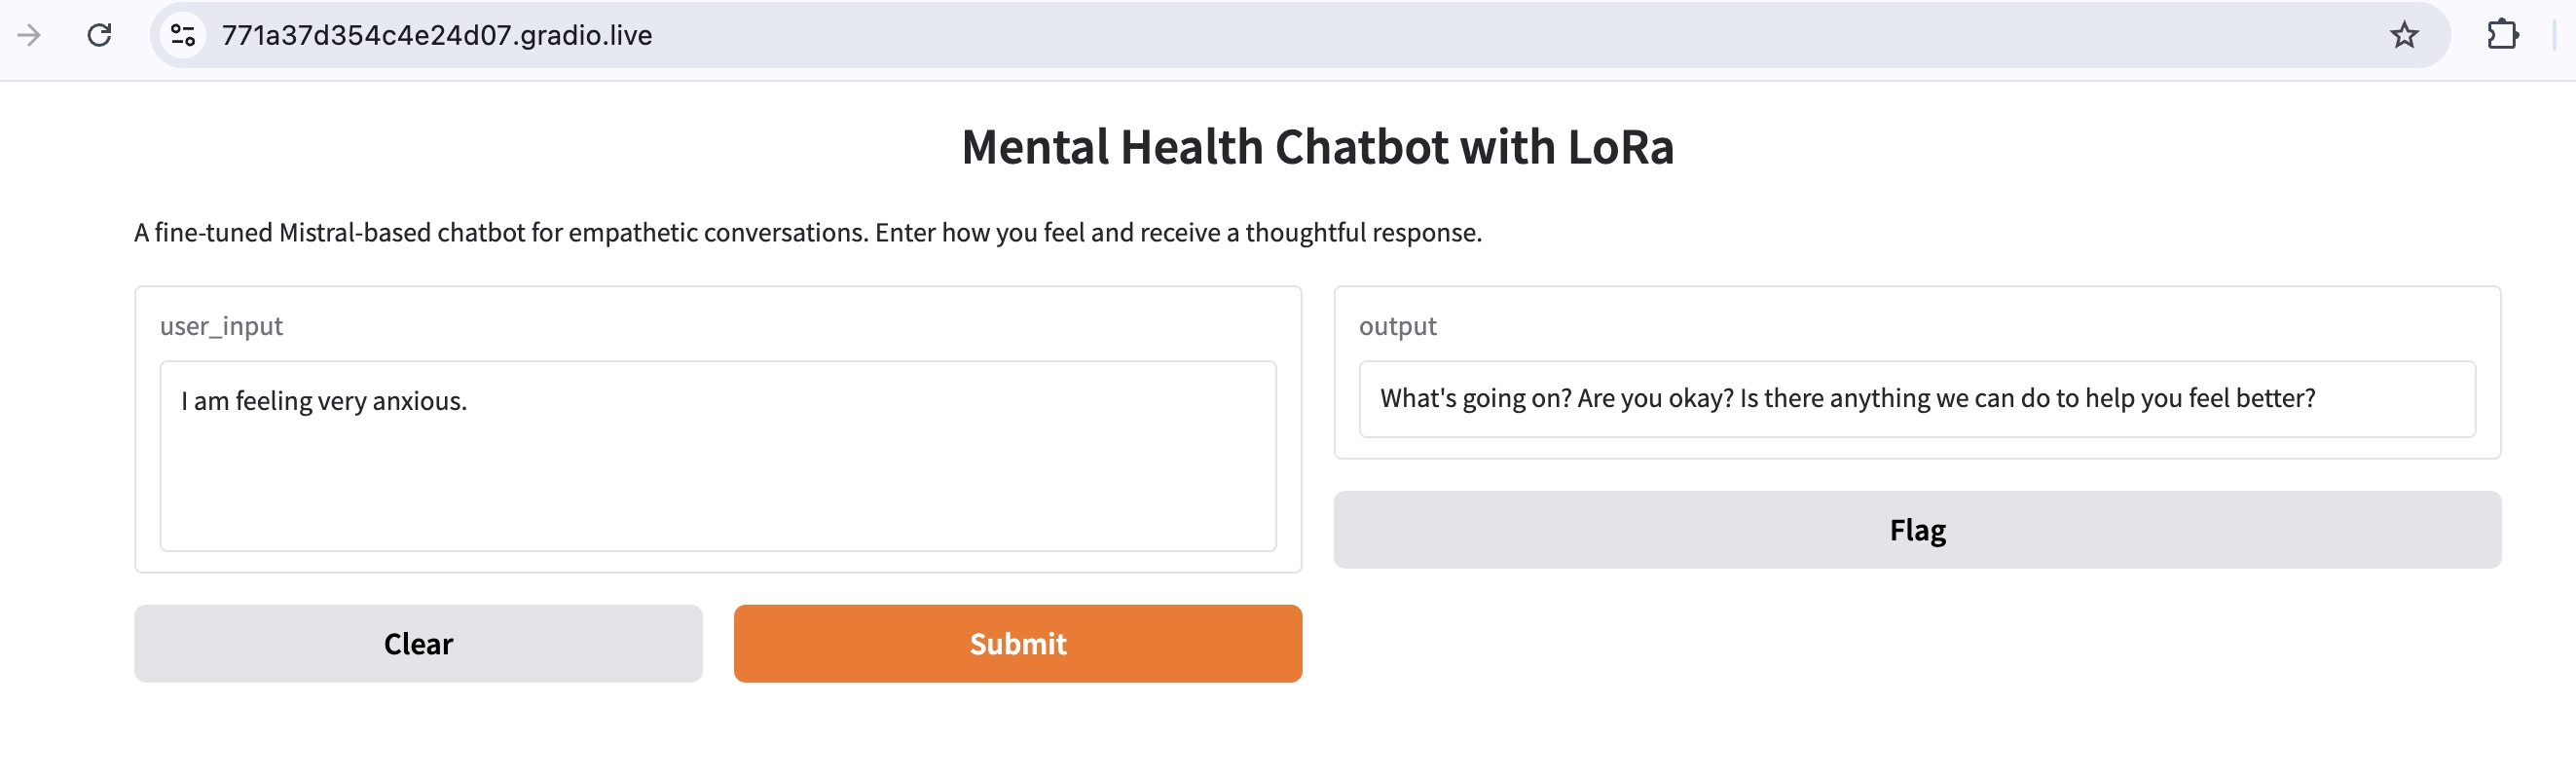
\includegraphics[width=0.8\textwidth]{chatbotwithlora.jpeg}
    \caption{Chatbot with LoRa}
    \label{fig:bot_lora}
\end{figure}
